\chapter{GROOVE}\label{app:B}

Descrevemos neste capítulo um trabalho de \citeonline{mathews_groove_1970}, GROOVE, ainda pouco observado por improvisadores de códigos. É o primeiro de trabalho de Mathews com reflexões nos aspectos performáticos. Não foi usado para ambientes de performance, mas a peça \emph{The expanding universe} da compositora Laurie \citeonline{spiegel_expanding_1975} foi considerada como exemplar por sua execução instrumental e disponibilidade \emph{online}.

GROOVE, ou \emph{Generated Real-time Operations On Voltage-controlled Equipment} foi um computador desenvolvido na Bell Labs por \cite{mathews_groove_1970}. Alex \citeonline{di_nunzio_genesi_2010} discute como um precedente direto do família de \emph{softwares} MUSIC N\footnote{Desenvolvidos a partir de 1957. As versões \emph{softwares} MUSIC I, II, III, IV, IV-B, IV-BF, V (que passou por modificações no IRCAM), MUSIC 360, MUSIC 11 acarretaram no desenvolvimento do \emph{software} CSound, disponível em \url{https://csound.github.io/}.}.

Seu desenvolvimento iniciou em 1968 na \emph{Bell Labs}. Segundo o próprio Mathews, o funcionamento do sistema oferece algumas possibilidades a partir de três conceitos: \emph{criação}, \emph{retroalimentação} e \emph{ciberficação}. O primeiro conceito foi implementado com um sistema de arquivos, onde as funções criadas no processo criativo são memorizadas, e podem ser editadas. O segundo conceito se relaciona com o terceiro:

\traduzcitacao{
O GROOVE provê oportunidades para uma retroalimentação imediata de observações dos efeitos das funções temporais para as entradas do computador, que compõem a função. No modo de composição do sistema GROOVE, um ser humano está em um ciclo de retroalimentação, como mostrado na figura 1 $[$\autoref{fig:groove_sistema}$]$. Assim ele é capaz de modificar as funções instantâneamente como um resultado de suas observações daqueles efeitos
}
{
GROOVE provides opportunity for immediate feedback from observations of the effects of time functions to computer inputs which compose the function. In the compose mode of the GROOVE system, a human beign is in the feedback loop (\ldots) Thus he is able to modify the functions instanteneously as a result of his observations of their effects.
}
{p.~715}{mathews_groove_1970}

\begin{figure}
\begin{center}
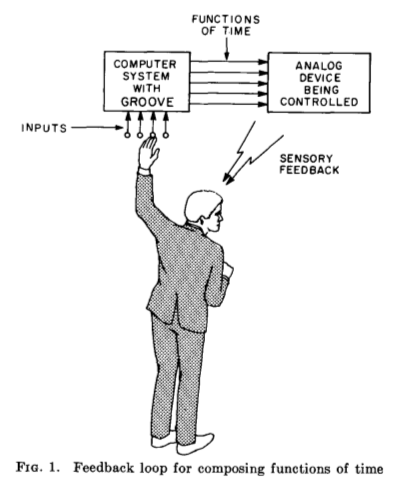
\includegraphics[scale=0.618]{./imagens/GROOVE.png}
\caption{Esquema de concepção do projeto GROOVE. \textbf{Fonte}: \cite{mathews_groove_1970}.}
\label{fig:groove_sistema}
\end{center}
\end{figure} 

O terceiro conceito observa a existência de uma relação entre um humano e uma máquina. Mathews descreve-o como uma \emph{engenharia humana}. Esta engenharia consistiu na observação de um tempo diferencial entre o que o(a) musicista cria e o que edita:

\traduzcitacao{
O conceito final é mais nebuloso. Desde que o GROOVE é um sistema homem-máquina, a engenharia humana do sistema foi a mais importante. Por exemplo, nós descobrimos que o controle do programa de tempo necessita ser bastante diferente para a composição do que para a edição, e o programa foi modificado de acordo. (\ldots) O intérprete de computador não deve tentar definir todo o som em tempo real. Ao invés, o computador deve ter uma partitura e o intérprete deve influenciar a forma como a partitura é tocada. Seus modos de influência podem ser mais variados do que aqueles que um regente convencional, que pode principalmente controloar o tempo, intensidade, e estilo
}
{
The final concept is more nebulous. Since GROOVE is a man-computer system, the human engeneering of the system is most important. For example, we discovered that the control of the program time needs to be quite different for composing than for editing, and the program was modiffied accordingly. (\ldots) The computer performer should not attempt to define the entire sound in real-time. Instead, the computer should have a score and the performer should influence the way in which the score is played. His modes of influence can be much more varied than that a conventional conductor who primarily controls tempo, loudness, and style.
}
{p.~715-716}{mathews_groove_1970}

Como exemplo , selecionamos uma descrição da compositora Laurie \citeonline{spiegel_expanding_1975} (ver \autoref{fig:groove}) para sumarizar as características do GROOVE, durante a produção de \emph{The Expanding Universe} \footnote{Disponível em \url{https://www.youtube.com/watch?v=dYUZmsfm4Ww}.}, entre as salas 2D-506 da Bell Labs (contendo o computador DDP-224) e a sala analógica 2D-562 (laboratório de Mathews). A ``performance'' da obra era realizada, com a programação de funções temporais e a manipulação de parâmetros dessas funções através de dispositivos físicos:

\begin{citacao}
Todas as músicas no GROOVE eram representadas na memória digital como funções abstratas do tempo, séries paralelas de dois pontos, cada ponto sendo um instante no tempo e um valor instantâneo. A taxa de amostragem para essas funções, usada principalmente como controle de voltagem, era cronometrada por um grande e antiquado oscilador analógico que era normalmente fixado em 100 Hertz, cada ciclo do oscilador pulsando à frente do código, o computador lia, em cada uma das funções, naquele ponto do tempo, todos dispositivos de entrada e executava todas amostras. (\ldots) Tínhamos uma pequena caixa com 4 potenciômetros e quatro chaves (alternadores fixados onde você os colocava) e dois botões de disparo.\footnote{Tradução de \emph{All music in GROOVE was represented in digital memory as abstract functions of time, parallel series of point pairs, each point being an instant in time and an instantaneous value. The sampling rate for these functions, which would be used mostly as control voltages, was clocked by a big old-fashioned analog oscillator that was usually set to 100 Hertz, each cycle of the oscillator pulsing one run through the code, the computer reading all of the real time input devices and playing of all of the samples at that time point in each of the time functions. (\ldots)  We had a small box with 4 knobs, 4 set switches (toggles that stay where you put them) and 2 momentary-contact push buttons on it.}}
\end{citacao}

\begin{figure}[!h]
  \begin{center}
  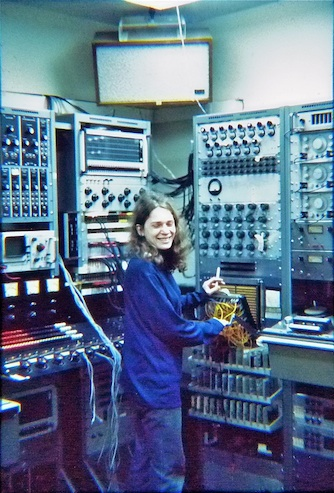
\includegraphics[scale=0.618]{./imagens/spiegel.jpg}
  \caption{\small Laurie Spiegel configurando a saída analógica do GROOVE, durante a produção de \emph{The Expanding Universe}. \textbf{Fonte}: \cite{spiegel_expanding_1975}.}
  \label{fig:groove}
  \end{center}
\end{figure}

Embora não declare ser uma peça minimalista, a descrição de \emph{The Expanding Universe} considera, de maneira asséptica, os fenômenos psicoacústicos como elementos composicionais. Por exemplo, a utilização da continuidade progressiva de sons (ou \emph{drones} transitórios) como elemento criativo permite, segundo a compositora, à sensibilização do ouvido, o que não seria possível na música minimalista instrumental:

\begin{citacao}
 A violência da perturbação sonora, disjunção, descontinuidade e mudanças súbitas desanitizam o ouvinte e nos afastam, de forma que não estamos mais abertos aos sons mais sutis. Mas com continuidade e gentileza, o ouvido se torna re-sensibilizado para mais e mais fenômenos auditoriais sutis dentro do som que estamos imersos. Em vez de sermos arrastados, como nas cascatas de muitas notas executadas em blocos de tempo que mudam repentinamente, tal como tantas vezes consite a música "minimalista", abrimos nossos ouvidos mais e mais para os fenômenos que nos envolvem. Isto também não é música ambiente, um termo que veio a ser usado alguns anos depois. Esta é música para atenção concentrada, uma experiência musical do através, pensando que, lógico, existe também um pano de fundo. \footnote{Tradução de\emph{The violence of sonic disruption, disjunction, discontinuity and sudden change desensitizes the listener and pushes us away so we are no longer open to the subtlest sounds. But with continuity and gentleness, the ear becomes increasingly re-sensitized to more and more subtle auditory phenomena within the sound that immerses us. Instead of being swept along, as with cascades of many running notes in suddenly-changing blocks of time, such as “minimalist” music so often consists of, we open up our ears more and more to the more minute phenomena that envelope us. This is also not “ambient music”, a term that came into use some years later. This is music for concentrated attention, a through-composed musical experience, though of course it also can be background.}}
\end{citacao}

Nesta citação podemos sumarizar um conceito para o \emph{live coding}: Música como um Processo Gradual \cfcite{reich_music_1968}. Porém, o significado de processo pode ser desenvolvido infinitamente. Isso não será realizado. O Processo para Spiegel é diverso daquele considerado no \emph{live coding}, e uma digressão desta pode afastar demais o foco do trabalho principal. Para compreesão deste termo, será necessário explorar outros aspectos correlacionados no decorrer deste trabalho.

Para finalizar esta sessão, a figura \autoref{fig:groove} sugere um conceito rotineiro para o \emph{live coder}. Esta rotina é uma atividade constante de improvisação códigos para aquisição de destreza para uma performance. \citeonline{iazzetta_musica_2009,soares_luteria_2015} lembram que esta atividade, de codificar como se construísse um instrumento musical, se caracteriza por sua conexão com a esfera composicional, nomeado \emph{luteria composicional}.